\documentclass{beamer}

\usepackage[british]{babel}
\usepackage{graphicx,hyperref,ru,url}
\usepackage{algorithm}
\usepackage{algpseudocode}
\usepackage{subcaption}
\usepackage{ragged2e} % Add this in preamble
\usepackage[center]{caption}


\def\newblock{\hskip .11em plus .33em minus .07em}
\captionsetup{justification = raggedright, singlelinecheck = false}
\captionsetup[subfigure]{justification=centering,singlelinecheck=false}

\definecolor{blueone}{RGB}{26,123,242}
\setbeamercolor{titlelike}{bg=blueone}

\makeatother

\setbeamertemplate{section in toc}
{\leavevmode\leftskip=5ex%
  \llap{%
    \usebeamerfont*{section number projected}%
    \usebeamercolor{section number projected}%
    \begin{pgfpicture}{-1ex}{0ex}{2.7ex}{4ex}
      \color{bg}
      \pgfpathcircle{\pgfpoint{0pt}{.8ex}}{1.9ex}
      \pgfusepath{fill}
      \pgftext[base]{\color{fg}\inserttocsectionnumber}
    \end{pgfpicture}\kern1.25ex%
  }%
  \inserttocsection\par}
\setbeamertemplate{subsection in toc}
  {\leavevmode\leftskip=2em$\bullet$\hskip1em\inserttocsubsection\par}
 
\setbeamertemplate{frametitle continuation}{}  
% The title of the presentation:
%  - first a short version which is visible at the bottom of each slide;
%  - second the full title shown on the title slide;
\title{AI-POWERED CODE DOCUMENT GENERATOR}

% The author(s) of the presentation:
%  - again first a short version to be displayed at the bottom;
%  - next the full list of authors, which may include contact information;

\author{\textbf{ARYA K A} \\ \textit{MCA S4\\ TCR24MCA-2020\\} \vspace{0.6cm}     
    Main Project  \\ 
 \vspace{13mm}     
    Guided By: \\
 \textbf{Sreejith V P} \\
    \\
    \vspace{0.3cm}
    Department of Computer Applications\\
    Government Engineering College, Thrissur, Kerala
}


% Add a date and possibly the name of the event to the slides
%  - again first a short version to be shown at the bottom of each slide
%  - second the full date and event name for the title slide
\date[GEC Thrissur]{}
\setbeamertemplate{caption}[numbered]
\begin{document}

\begin{frame}[plain]
  \titlepage
  
\end{frame}


%\setbeamertemplate{section in toc}[circle]
\begin{frame}[allowframebreaks]{Outline}
% --- Formatting for uniform spacing ---
\setlength{\parskip}{1pt}   % space between paragraphs
\setlength{\itemsep}{2pt}   % space between items

% --- Show numbered sections only ---
\tableofcontents[
    sectionstyle=show/show,     % show all section numbers
    subsectionstyle=hide,       % hide subsections (clean look)
    subsubsectionstyle=hide
]
\end{frame}



% You can reveal the parts of a slide one at a time
% with the \pause command:
\section{Introduction}

\begin{frame}{Introduction}

\begin{itemize}
  \justifying
  \item Rapid growth of software systems has increased project complexity.

\item Code documentation is essential for improving readability, collaboration, and long-term maintenance.

\item Manual documentation is often outdated and incomplete.

\item Frequent code changes make documentation difficult to maintain.

\item Abstract Syntax Tree (AST) technique is a structured tree representation of source code that captures its syntactic elements such as functions, variables, and control structures.

\item Combining AST-based code analysis with code-specific Large Language Models (LLMs) enables automatic and accurate documentation generation.

  
\end{itemize}

\end{frame}

\begin{frame}{Introduction}


\item \textbf{Objectives:}
\begin{itemize}
\justifying
    The objective of this project is to develop an AI-powered system that automatically generates structured and accurate documentation from source code. By using AST based code analysis and a code-specific LLM, the system aims to reduce manual documentation effort, handle frequent code changes, and improve software readability and maintainability.




    
    
\end{itemize}
\end{frame}


\section{Literature Review}

%------------------ Paper 1 ------------------%
\begin{frame}{Literature Review}
\justifying
\hypertarget{lit1}{}
\begin{block}{Khan, A., Li, W., and Zhang, Y.,
“CodeDocAgent: Leveraging Large Language Models for Accurate and Contextual Code Documentation,”
\textit{IEEE Transactions on Software Engineering}, 2025.}
\end{block}

\begin{itemize}
\justifying
    \item Proposed a repository-level documentation generation framework using LLMs.
    \item Integrated AST analysis with project structure and dependency relationships.
    \item Generated contextual and structured documentation rather than isolated code comments.
    \item \textbf{Observation:} Highlights the effectiveness of combining structural code analysis with LLMs for accurate software documentation.
\end{itemize}
\end{frame}

%------------------ Paper 2 ------------------%
\begin{frame}{Literature Review}
\justifying
\hypertarget{lit2}{}
\begin{block}{Zhang, M., Chen, R., and Wang, L.,
“AI-Driven Automated Software Documentation Generation for Enhanced Development Productivity,”
\textit{Journal of Systems and Software}, 2024.}
\end{block}

\begin{itemize}
\justifying
    \item Treated software documentation generation as a code-to-text translation task.
\item Employed transformer-based models like GPT-2 and RoBERTa for automated documentation generation.
\item Achieved significant performance improvements through fine-tuning, where GPT-2 obtained an accuracy of 74.37\%, while RoBERTa achieved a superior accuracy of 99.94\%.
\item \textbf{Observation:} The results demonstrate the strong potential of AI-based transformer models for automated documentation generation

\end{itemize}
\end{frame}

%------------------ Paper 3 ------------------%
\begin{frame}{Literature Review}
\justifying
\hypertarget{lit3}{}
\begin{block}{Khan, M. R. I. and Uddin, G.,
“Combining Contexts from Multiple Sources for Documentation-Specific Code Example Generation,”
\textit{Proc. IEEE International Conference on Software Analysis, Evolution and Reengineering (SANER)}, 2023.}
\end{block}

\begin{itemize}
\justifying
    \item Proposed a framework for generating documentation-specific code examples using LLMs.
    \item Combined source code, existing documentation, and compiler error logs as contextual inputs.
    \item Utilized an iterative error-feedback mechanism to improve example correctness.
    \item \textbf{Observation:} Shows the importance of multi-source context fusion for improving documentation usability.
\end{itemize}
\end{frame}

\begin{frame}{Literature Review}
\justifying
\hypertarget{lit5}{}
\begin{block}{Zhu, Y., Zhao, X., Li, X., Zou, Y., Yuan, H., Wang, Y., and Xie, B.,
“RepoSummary: Feature-Oriented Summarization and Documentation Generation for Code Repositories,”
\textit{ACM Transactions on Software Engineering and Methodology}, 2025.}
\end{block}

\begin{itemize}
\justifying
    \item Proposed a feature-oriented approach for repository-level code summarization and documentation generation.
    \item Performed hierarchical analysis using file-level and method-level dependency relationships.
    \item Employed LLM to generate feature descriptions while preserving traceability links.
    \item \textbf{Observation:} Produces well-structured and feature-centric documentation with improved traceability; however, the approach involves complex clustering and high computational overhead.
\end{itemize}
\end{frame}
\begin{frame}{Literature Review}
\justifying
\hypertarget{lit4}{}
\begin{block}{Wang, W., Zhang, Y., Sui, Y., Wan, Y., Zhao, Z., Wu, J., Yu, P. S., and Xu, G.,
“Reinforcement-Learning-Guided Source Code Summarization using Hierarchical Attention,”
\textit{IEEE/ACM International Conference on Software Engineering}, 2020.}
\end{block}

\begin{itemize}
\justifying
    \item Proposed a source code summarization model guided by reinforcement learning.
    \item Utilized a hierarchical attention mechanism to capture both lexical and structural code information.
    \item Optimized summary generation using evaluation metrics such as BLEU as reinforcement rewards.
    \item \textbf{Observation:} Improves code summarization quality with 22\%--45\% BLEU-1 improvement, but is limited to method-level summarization.

\end{itemize}
\end{frame}
\begin{frame}{Literature Review}

\begin{tabular}{|p{1.8cm}|p{2.2cm}|p{6.2cm}|}
\hline
\textbf{Author} & \textbf{Approach} & \textbf{Brief Observation} \\
\hline

Khan et al. (2025) &
LLM + AST &
Structural code analysis combined with LLMs improves contextual documentation accuracy. \\
\hline

Zhang et al. (2024) &
Transformer Code-to-Text &
Transformer models achieve high accuracy in automated documentation generation. \\
\hline

Khan et al. (2023) &
Multi-source Context LLM &
Combining code, documentation, and compiler feedback improves example correctness. \\
\hline

Zhu et al. (2025) &
Feature-oriented Analysis &
Feature-level summarization enhances coherence of repository documentation. \\
\hline

Wang et al. (2020) &
RL-guided &
Reinforcement learning improves code summarization quality. \\
\hline

\end{tabular}





\end{frame}


\section{Existing Systems}

\begin{frame}{Existing Systems}
\begin{itemize}
\justifying
\item Rely mostly on manual or semi-automated software documentation processes.
\item Traditional documentation tools generate static comments or templates with limited context.
\item NLP-based summarization approaches lack deep understanding of program structure.
\item Fail to capture inter-file dependencies and repository-level relationships.

\end{itemize}
\end{frame}


\section{Proposed System}

\begin{frame}{Proposed System}
\begin{itemize}
\justifying
\item An AI-powered framework for automatic and contextual software documentation generation.
\item Extracts textual features and structural information using AST analysis.
\item Models code relationships using graph-based dependency representation.
\item Integrates extracted features and feeds them into a code specialized LLM.
\item Generates accurate, structured, and repository-level documentation with minimal human intervention.
\end{itemize}
\end{frame}




\section{Requirements Specification}
\begin{frame}{Requirements Specification}
    Hardware Requirements
    \begin{itemize}
    \justifying
    \item \textbf{Processor}: Intel i5 (8th Gen or higher) / AMD Ryzen 5 or higher
    \item \textbf{Memory}: Minimum 8 GB RAM
    \item \textbf{Storage}:50-100 GB free disk space
    % \item \textbf{Display}: 1366 $\times$ 768 resolution or higher
    

\end{itemize}
\end{frame}

\begin{frame}{Requirements Specification}
     Software Development Requirements
     \begin{itemize}
     \justifying
        \item \textbf{Operating System}: Windows 10 / Ubuntu 20.04 LTS / macOS
    \item \textbf{Back End}: Python 3.8 or higher
    \item \textbf{IDE Used}: Visual Studio Code
    \item \textbf{Version Control}: Git
    \item \textbf{Development Tools and Frameworks}:
    \begin{itemize}
        \item Tree-sitter
        \item Code-specialized Large Language Model
    \end{itemize}
\end{itemize}
\end{frame}
% \begin{frame}{Requirements Specification}
% \begin{itemize}
%      \justifying
%      \item \textbf{Graph Processing Libraries}: NetworkX
%      \item \textbf{Data Handling Libraries}: NumPy, Pandas
%      \item \textbf{Visualization Tools}: Matplotlib
% \end{itemize}
% \end{frame}


\begin{frame}[allowframebreaks]{Requirements Specification}
Functional Requirements
\begin{itemize}
\justifying
\item \textbf{User Interface:} The system shall provide a simple and intuitive interface for documentation generation.
% \item \textbf{Project Selection:} The system shall allow users to select a local source code directory or repository.
\item \textbf{Source Code Input:} The system shall accept software projects as local folders or version-controlled repositories.
\item \textbf{Code Parsing:} The system shall parse source code files using AST generation.
\item \textbf{Feature Extraction:} The system shall extract structured features such as modules, classes, functions, imports, and dependencies.




\item \textbf{LLM-Based Generation:} The system shall use a code-speciali-zed LLM to generate documentation.
\item \textbf{Documentation Output:} The system shall generate structured documentation including project overview, architecture, API, and module-level explanations.
\begin{itemize}
    \item \textbf{README.md}
    \item \textbf{architecture\_overview.md} 
    \item \textbf{recent\_changes.md} 
    \item \textbf{modules/*.md} – 
\end{itemize}
\end{itemize}


\end{frame} 
\begin{frame}{Requirements Specification}
Non-Functional Requirements
\begin{itemize}
\justifying
    \item \textbf{Performance:} The system shall generate documentation efficiently within acceptable response time.
\item \textbf{Scalability:} The system shall handle projects of different sizes and complexities.
\item \textbf{Usability:} The system shall provide a simple and user-friendly interface.
\item \textbf{Reliability:} The system shall consistently produce accurate documentation without failures.
\end{itemize}
\end{frame}

\section{Input and Output}

\begin{frame}{Input and Output}
\begin{itemize}
\justifying
\item \textbf{Input:} Single source code file or a full project directory (local or version-controlled).
\item \textbf{Input Format:} Source code files written in supported programming languages(Python, Java, C, C++, C\#, JavaScript, TypeScript, Go, Rust, Ruby, PHP, Kotlin).
\item \textbf{Output:} Automatically generated software documentation.
\item \textbf{Output Format:} Structured documentation which includes README, recent changes, architecture, and module descriptions.
\end{itemize}
\end{frame}


\section{System Architecture}
\begin{frame}{System Architecture}
\begin{figure}
                \centering
                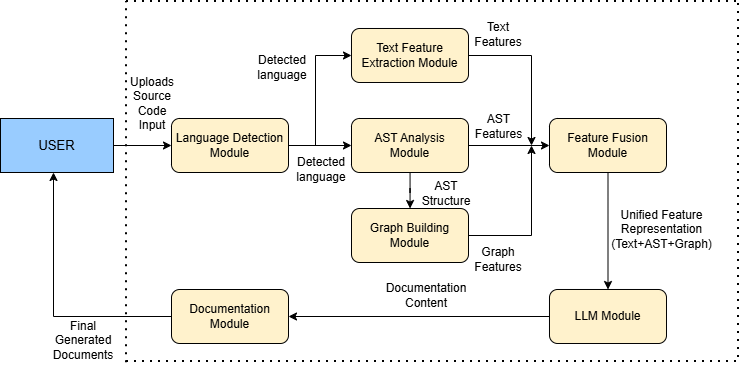
\includegraphics[width=0.9\linewidth]{Untitled Diagram-Page-2.drawio (3).png}
                                \captionsetup{justification=centering}

                \caption{Architecture Diagram}
                \label{fig:placeholder}
            \end{figure}
\end{frame}

\section{Data Flow Diagram}
\begin{frame}{Data Flow Diagrams}
\begin{figure}
            \centering
            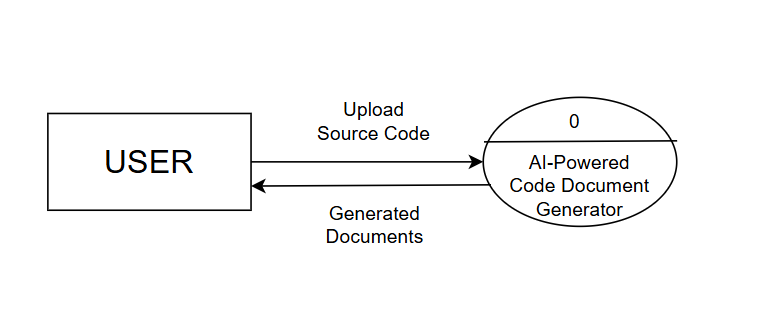
\includegraphics[width=0.9\linewidth]{Screenshot 2026-03-11 152839.png}
                          \captionsetup{justification=centering}
                        \caption{Level 0 DFD}
            \label{fig:placeholder}
        \end{figure}   
\end{frame}

\begin{frame}{Data Flow Diagrams}
\begin{figure}
            \centering
            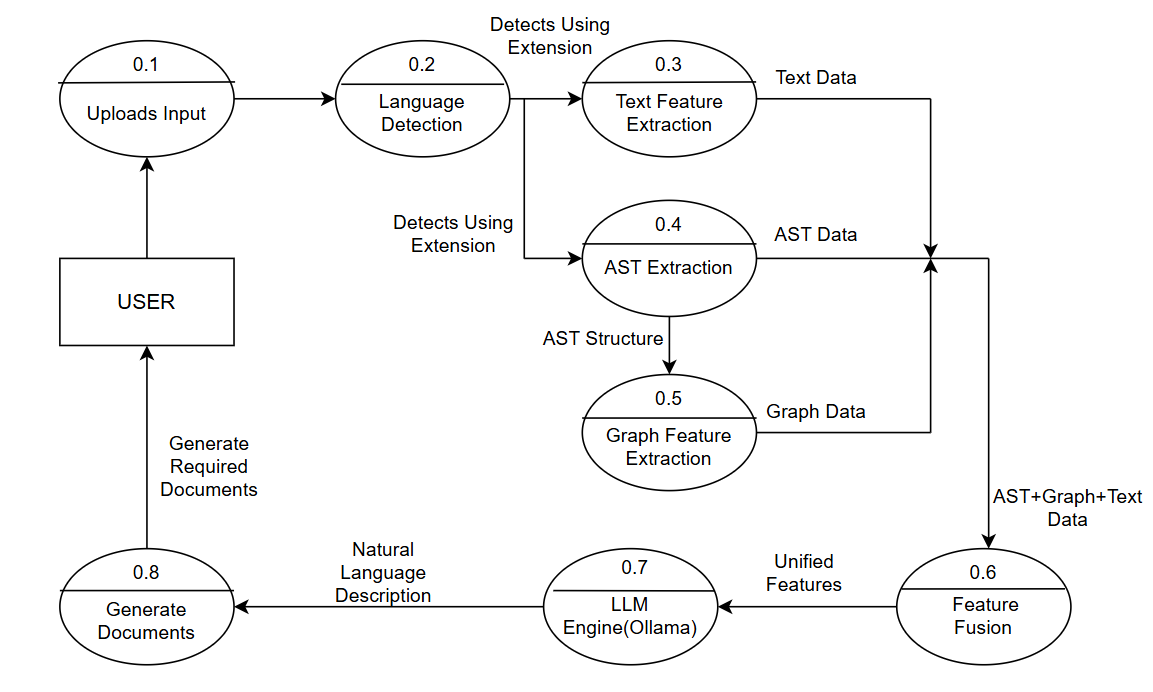
\includegraphics[width=0.9\linewidth]{Screenshot 2026-03-11 142330.png}
                          \captionsetup{justification=centering}
            \caption{Level 1 DFD}
            \label{fig:placeholder}
        \end{figure}
\end{frame}

 \section{System Modules}
\begin{frame}[allowframebreaks]{System Modules}
\begin{itemize}
    \justifying
    \item \textbf{User Interface Module:}  
    Provides an interface for uploading source code files, project folders, or repositories and viewing generated documentation.

    

    \item \textbf{Language Detection Module:}  
    Detects the programming language of each source file to enable accurate parsing.

    \item \textbf{AST Analysis Module:}  
   Generates an Abstract Syntax Tree to extract structural components like classes, functions, variables, and dependencies.



    \item \textbf{Text Feature Extraction Module:}  
    Computes metrics such as lines of code, tokens, comments, and identifiers to assess code size and complexity.



    \item \textbf{Graph Building Module:}  
    Builds graph representations with nodes and edges to model relationships like imports and definitions.

    \item \textbf{Feature Fusion Module:}  
    Combines structural, textual, and graph-based features into a unified representation.

    \item \textbf{LLM Engine Module:}  
    Uses combined features to generate clear and structured documentation of the codebase.


    \item \textbf{Documentation Output Module:}  
    Organizes the generated content into structured formats.


\end{itemize}
\end{frame}

% \begin{frame}[allowframebreaks]{Completed Modules}
% \begin{itemize}
% \justifying
%     \item \textbf{Language Detection Module:} Detects programming languages of source files.
%     \item \textbf{AST Analysis Module:} Generates Abstract Syntax Trees to extract classes, functions, variables, and dependencies.\\
%           \textit{Note: Currently AST works only on some languages, not all 13 supported languages.}
%     \item \textbf{Text Feature Extraction Module:} Computes code metrics like lines of code, tokens, comments, and identifiers.
%     \item \textbf{Graph Building Module:} Builds graph representations with nodes and edges for imports and definitions.
%     \item \textbf{Feature Fusion Module:} Combines structural, textual, and graph features into a unified representation.
%     \item \textbf{Vector Store Module:} Converts features into embeddings and stores them in a vector database.
%     \item \textbf{LLM Engine Module:} Generates structured documentation from contextual embeddings.
%     \item \textbf{Documentation Output Module:} Organizes generated content into Markdown or structured formats.
% \end{itemize}
% \end{frame}
% \begin{frame}{Next Steps / Improvements}
% \begin{itemize}
% \justifying
%     \item Develop a frontend for uploading files and viewing documentation.
%     \item Improve AST extraction to support all 13 languages.
%     \item Enable module-wise and global documentation generation.
%     \item Add Git repository support for complete project analysis.
    
    
%     \item Fine-tune LLM explanations for clarity.
% \end{itemize}
% \end{frame}
\section{Implementation}
\begin{frame}[allowframebreaks]{Implementation}
\begin{itemize}
\justifying
\item Successfully implemented all the important modules
    of the system, i.e, Language Detection, AST Analysis,
    Text Feature Extraction, Graph Building, Feature Fusion,
   and Documentation Output.
    \item Detects programming
    language using file extension mapping.
    \item Tree-sitter parses source
    code to extract classes, functions, and dependencies.
    \item Computes code
    metrics such as lines of code, tokens, and identifiers.
    \item  Models inter-file
    relationships using node-edge graph representation.
    \item  Combines structural,
    textual, and graph features into a unified representation.
    \item Ollama generates structured
    natural language documentation from fused features.
    \item Produces Markdown
    files — README, architecture overview,recent changes and module docs.
\end{itemize}
\end{frame}
\section{Results}
\begin{frame}{Results}
\begin{itemize}
\justifying
    \item System automates generation of structured
    documentation from source code.
    \item Supports multiple programming languages with
    an easy-to-use interface.
    \item Provides README, architecture overview,recent changes and
    detailed module-level documentation.
    \item Ensures accurate, and consistent
    documentation with minimal human effort.
\end{itemize}
\end{frame}
\begin{frame}{Results}
\begin{itemize}
    \begin{figure}
        \captionsetup{justification=centering}
        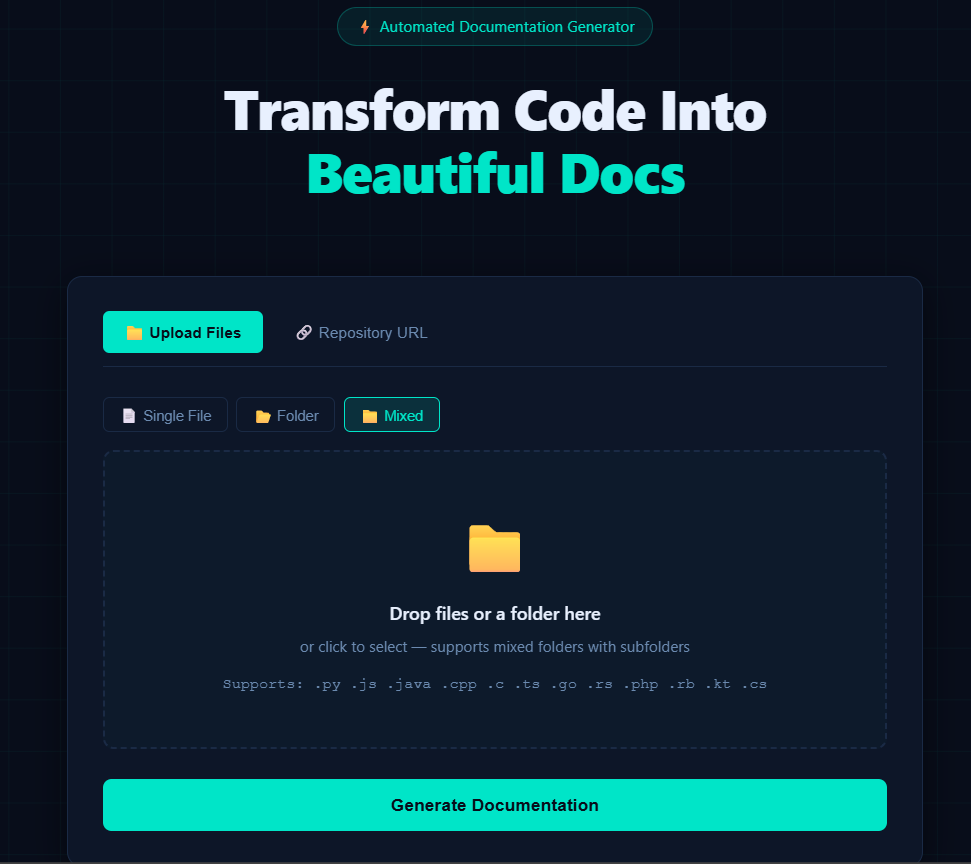
\includegraphics[width=0.7\linewidth]{Screenshot 2026-03-01 101625.png}
                                \caption{User Interface}
        \label{fig:enter-label}
    \end{figure}

\end{itemize}
\end{frame}


\begin{frame}{Results}
\begin{itemize}
    \begin{figure}
        \captionsetup{justification=centering}
        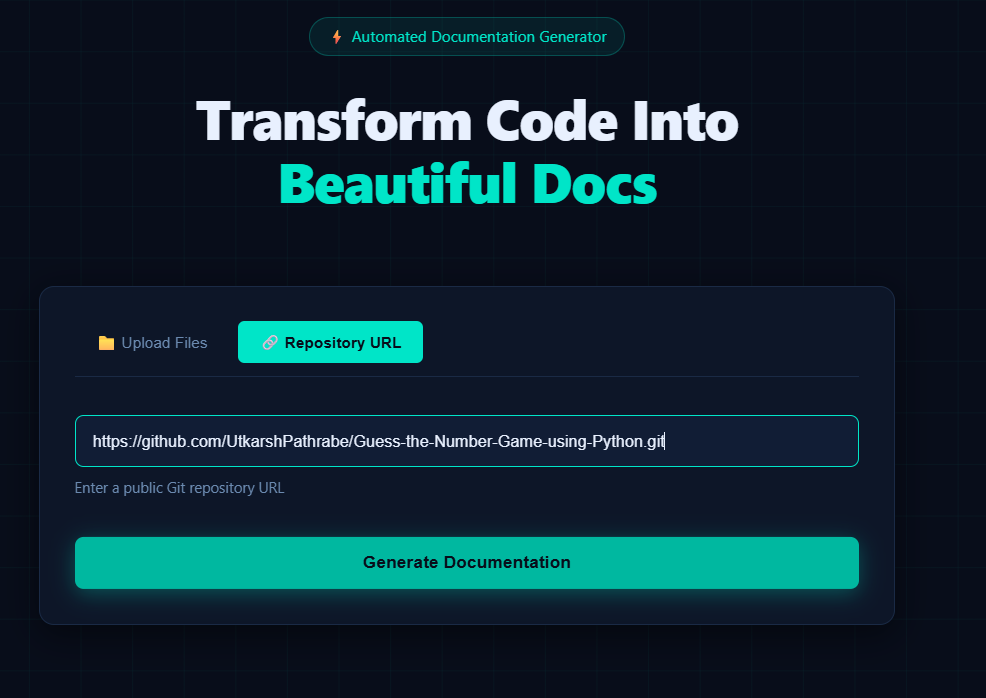
\includegraphics[width=0.7\linewidth]{Screenshot 2026-03-01 101806.png}
        \caption{Inputs uploading}
        \label{fig:enter-label}
    \end{figure}

\end{itemize}
\end{frame}

\begin{frame}{Results}
\begin{itemize}
    \begin{figure}
        \captionsetup{justification=centering}
        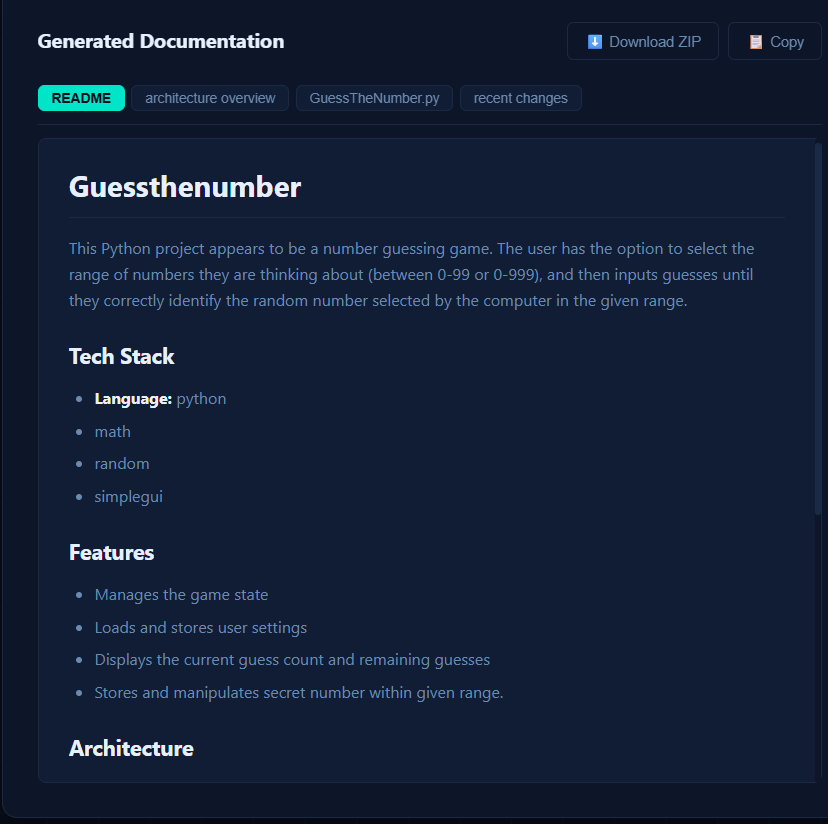
\includegraphics[width=0.5\linewidth]{Screenshot 2026-03-01 112430.png}
        \caption{Output-README.md}
        \label{fig:enter-label}
    \end{figure}

\end{itemize}
\end{frame}


\begin{frame}{Results}
\begin{itemize}
    \begin{figure}
        \captionsetup{justification=centering}
        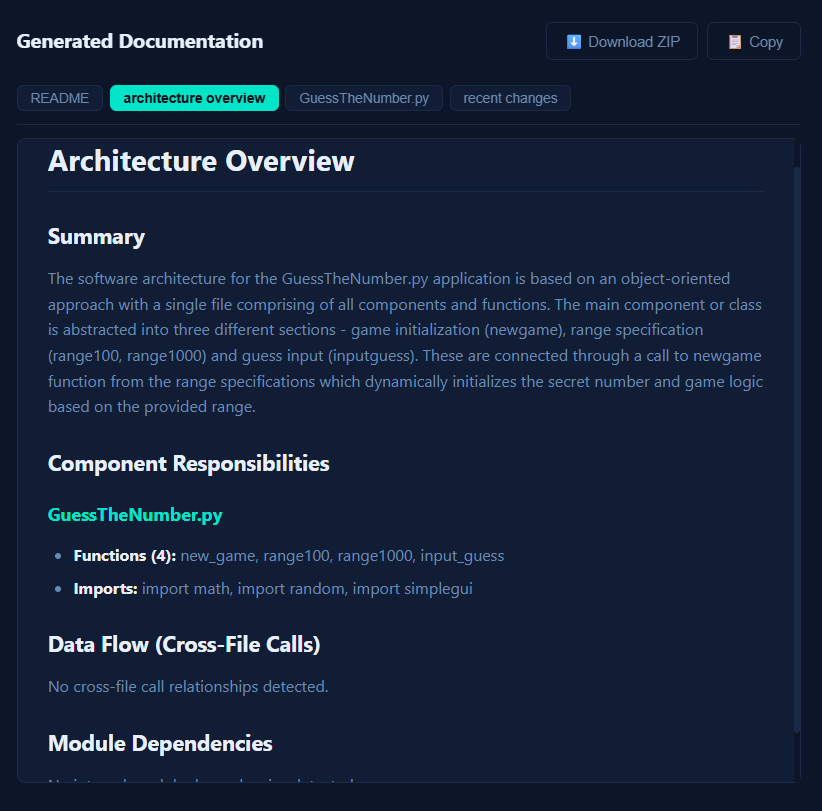
\includegraphics[width=0.5\linewidth]{Screenshot 2026-03-01 112444.png}
        \caption{Output-architecture$_$overview.md}
        \label{fig:enter-label}
    \end{figure}

\end{itemize}
\end{frame}
\begin{frame}{Results}
\begin{itemize}
    \begin{figure}
        \captionsetup{justification=centering}
        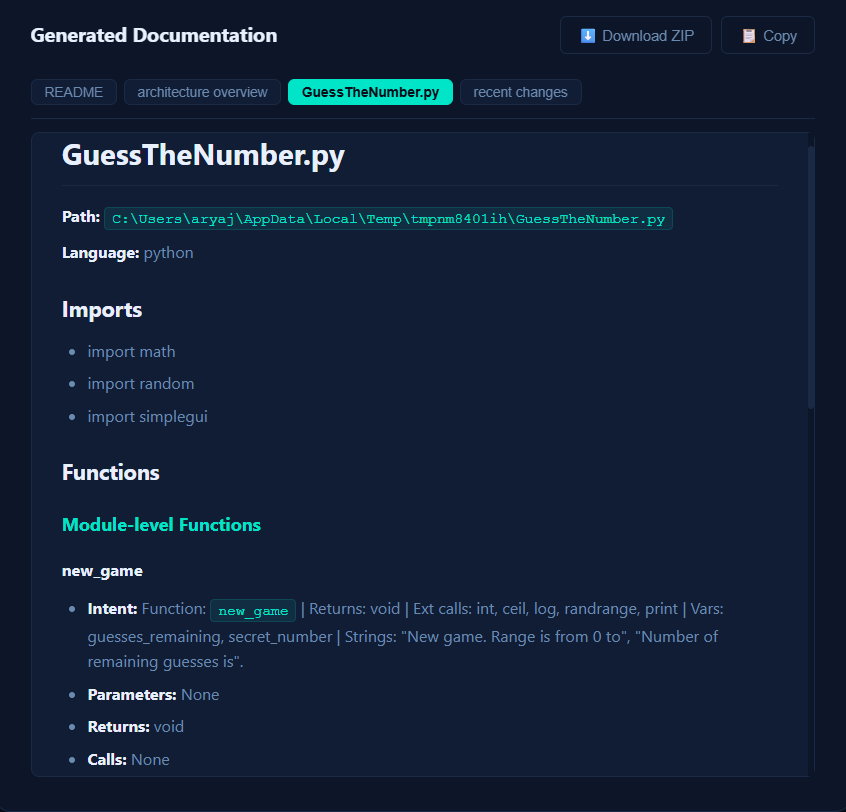
\includegraphics[width=0.5\linewidth]{Screenshot 2026-03-01 112456.png}
        \caption{Output-files.md}
        \label{fig:enter-label}
    \end{figure}

\end{itemize}
\end{frame}
\begin{frame}{Results}
\begin{itemize}
    \begin{figure}
        \captionsetup{justification=centering}
        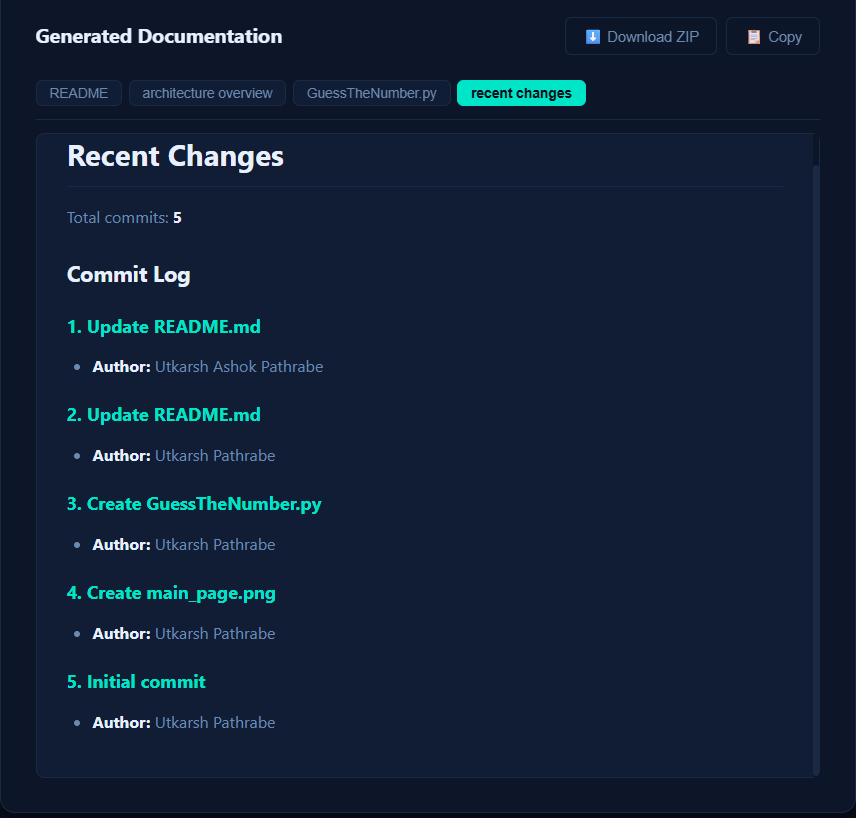
\includegraphics[width=0.5\linewidth]{Screenshot 2026-03-01 112509.png}
        \caption{Output-recent$_$changes.md}
        \label{fig:enter-label}
    \end{figure}

\end{itemize}
\end{frame}
% \begin{frame}
% \frametitle{Evaluation Metrics}

% \begin{itemize}
% \justifying
%     \item mAP: 0.54 — accurate external damage detection.


% \end{itemize}
% \end{frame}
\section{Future Enhancement}

% --- Slide 1 ---
\begin{frame}{Future Enhancement}
\justifying
\begin{itemize}
\justifying
    \item \textbf{Git Integration:} Automatically regenerate
    documentation on every commit for always up-to-date
    docs.
    
    \item \textbf{Multi-Language Expansion:} Extend support
    to additional languages such as Swift, Scala, and
    Haskell.
    \item \textbf{Interactive Q\&A:} Allow developers to
    query the codebase in natural language using the
    generated documentation as context.
   
\end{itemize}
\end{frame}

\section{Conclusion}
\begin{frame}{Conclusion}

\begin{itemize}
\justifying
    \item This project developed an AI-powered system that
    automatically generates structured and accurate
    documentation from source code using AST analysis
    and a code-specialized Large Language Model.

\item It reduces manual documentation effort and improves
    software readability, maintainability, and developer
    productivity.

\item Overall, the AI-Powered Code Document Generator
    demonstrates how AI can bridge the gap between complex
    codebases and clear, accessible software documentation.
\end{itemize}
\end{frame}

\section{References}
    \begin{frame}[allowframebreaks]{References}
    \setbeamertemplate{bibliography item}[text]
     \begin{thebibliography}{10}
  

\justifying
\bibitem{CodeDocAgent2025}
A. Khan, W. Li and Y. Zhang,
``CodeDocAgent: Leveraging Large Language Models for Accurate and Contextual Code Documentation,''
\emph{IEEE Transactions on Software Engineering},
 2025.

\bibitem{AIDocGen2024}
M. Zhang, R. Chen and L. Wang,
``AI-Driven Automated Software Documentation Generation for Enhanced Development Productivity,''
\emph{Journal of Systems and Software},
 2024.

\bibitem{ContextExample2023}
M. R. I. Khan and G. Uddin,
``Combining Contexts from Multiple Sources for Documentation-Specific Code Example Generation,''
in \emph{Proc. IEEE International Conference on Software Analysis, Evolution and Reengineering (SANER)},
2023.
\bibitem{RepoSummary2023}
Y. Zhu, X. Zhao, X. Li, Y. Zou, H. Yuan, Y. Wang and B. Xie,
``RepoSummary: Feature-Oriented Summarization and Documentation Generation for Code Repositories,''
in \emph{Proc. ACM/IEEE International Conference on Software Engineering (ICSE)},
2023.
\bibitem{RLCodesum2018}
W. Wang, Y. Zhang, Y. Sui, Y. Wan, Z. Zhao, J. Wu, P. S. Yu and G. Xu,
``Reinforcement-Learning-Guided Source Code Summarization using Hierarchical Attention,''
\emph{IEEE Transactions on Software Engineering},
 2020.




 \end{thebibliography}
\end{frame}

    



\section{Acknowledgement}  
\begin{frame}

\vspace{10pt}
\huge{\centerline{Thank You}}


%\textcolor{myNewColorA}{\Large{\centerline{E-mail: mhdnihan@gmail.com}}}

\end{frame}

\end{document}
